\section{AutoPas Software}

AutoPas is a C++ library specifically designed to optimize short-range particle simulations through dynamic algorithm selection. It acts as a black box, where users provide the specifications while the library handles the choice of the best suitable algorithm through auto tuning. By periodically evaluating various algorithms, AutoPas ensures that the most efficient configuration is applied as simulation conditions change. This adaptability is particularly useful for large-scale or dynamic simulations where optimal configurations may shift over time. Although AutoPas is primarily intended for node-level simulations, however it can be integrated into distributed systems. The library also includes example applications, such as the md-flexible framework, which will be used in the course of this thesis \parencite{gratl2019autopas}.


\subsection{Data layouts}

AutoPas supports two primary data layouts for storing particle information in memory: Array of Structures (AoS) and Structure of Arrays (SoA). In the AoS layout, each particle is represented as an object containing all its properties, such as position and force, stored together in memory. This arrangement allows for efficient cache utilization when accessing individual particles, but can limit vectorization efficiency. In contrast, the SoA layout separates particle properties into individual arrays, with each array containing data for all particles, enabling better vectorization by aligning data contiguously in memory. However, this layout may lead to less efficient cache usage when accessing properties of a single particle. The choice of data layout depends on the specific simulation requirements, as each has trade-offs in terms of memory access patterns and computational performance \parencite{gratl2019autopas}.

\subsection{Neighbor identification algorithms} \label{sec:neighbor_iden_algs}

During auto tuning AutoPas has to decide how to manage and store the particles of the simulation, and most importantly how to identify the neighboring particles to efficiently compute the pairwise forces. As shown in section \ref{sec:shortrange}, for each particle, the particles within the cut-off radius should be found, and the rest will be ignored. This process is repeated for every single particle in the container, and choosing the right Neighbor identification algorithm, is crucial when it comes to performance. Below, the four algorithms used in AutoPas are presented. These algorithms are implemented as containers in AutoPas, managing neighbor identification and the overall particle organization, including the selection of the data layout. 

\subsubsection{Direct Sum}

The straightforward, and thus naive, approach, is to calculate the distances from one particle to all other particles without utilizing any additional data structures. Instead, all particles are stored in a single cell, and for each particle, distances to all other particles are evaluated to determine whether they fall within the cutoff radius. Forces are only computed for pairs of particles within this radius. As illustrated in \hyperref[fig:directsum]{Figure \ref*{fig:directsum}}, the red particle represents the current particle, for which forces are being calculated, the red circle denotes the cutoff radius, and the arrows depict the interactions between the current particle and the others.

This method, while eliminating the complexity and overhead associated with data structures, is computationally inefficient. The calculation of pairwise forces results in a time complexity of \(O(n^2)\), where \(n\) is the number of particles \parencite{gratl2022n}. Although simple, this approach is only practical for simulations with a very small number of particles.


\subsubsection{Linked Cells}

This approach extends the Direct Sum method by dividing the simulation domain into cells, with each cell containing the particles within its boundaries. The cell dimensions are set to at least the cutoff radius. This ensures that short-range interactions are computed only between particles in the current cell and its eight neighboring cells, as depicted with blue in \hyperref[fig:linkedcells]{Figure \ref*{fig:linkedcells}}.

Because the cell size matches the cutoff radius, particles outside these neighboring cells are guaranteed to lie beyond the interaction range and can be excluded from force calculations. For homogeneous particle distributions, this reduces the computational complexity from \(O(n^2)\) to \(O(n)\) \parencite{knapek2007numerical}. Furthermore, Linked Cells improve cache efficiency by storing particles within the same cell contiguously in memory. Nonetheless, there is still overhead, since additional particles need to be evaluated to determine if they can be considered for force calculations.



\subsubsection{Verlet Lists}

The Verlet list method extends the Linked Cells algorithm by precomputing and storing neighbor lists or verlet lists for each particle. These lists include all particles within a cutoff radius \(r_c\) plus an additional buffer zone defined by the verlet skin factor \(s\), resulting in a search radius of \(r_c \cdot s\), illustrated with yellow in \hyperref[fig:verletlists]{Figure \ref*{fig:verletlists}}. This buffer ensures that fast-moving particles do not enter or leave the cutoff region unnoticed, allowing the neighbor lists to be reused for multiple iterations.

Constructing these lists involves evaluating only particles in nearby cells, improving runtime efficiency. During each iteration, distance checks are performed only for the stored neighbors, achieving a complexity of \(O(N)\) \parencite{yao2004improved}. While smaller buffer sizes reduce unnecessary calculations, they require more frequent updates to the lists, making the choice of \(s\) crucial for performance.

Verlet lists are particularly effective for systems with high particle densities. However, their lack of spatial locality can lead to inefficient memory access, resulting in poor cache performance and reduced vectorization efficiency \parencite{gratl2022n}.


\subsubsection{Verlet Cluster Lists}

Verlet Cluster Lists are built upon regular Verlet Lists by grouping particles into clusters rather than maintaining individual neighbor lists for each particle \hyperref[fig:verletclusters]{Figure \ref*{fig:verletclusters}}. This approach reduces memory overhead, as a single neighbor list is created for each cluster instead of one for every particle. The algorithm uses the observation that neighboring particles often share similar neighbor lists, allowing $M$ particles to be combined into a cluster. When two clusters are close, all interactions between the particles within these clusters are calculated. This optimization decreases the number of neighbor lists by a factor of $\frac{1}{M}$ \parencite{gratl2022n}, and enhances computational efficiency by enabling better vectorization. However, the increased search radius, can lead to additional distance calculations. Despite this, Verlet Cluster Lists are well-suited for large systems with high particle densities.

\begin{figure}[h!]
    \centering
    % First Figure
    \begin{subfigure}{0.22\textwidth}
        \centering
        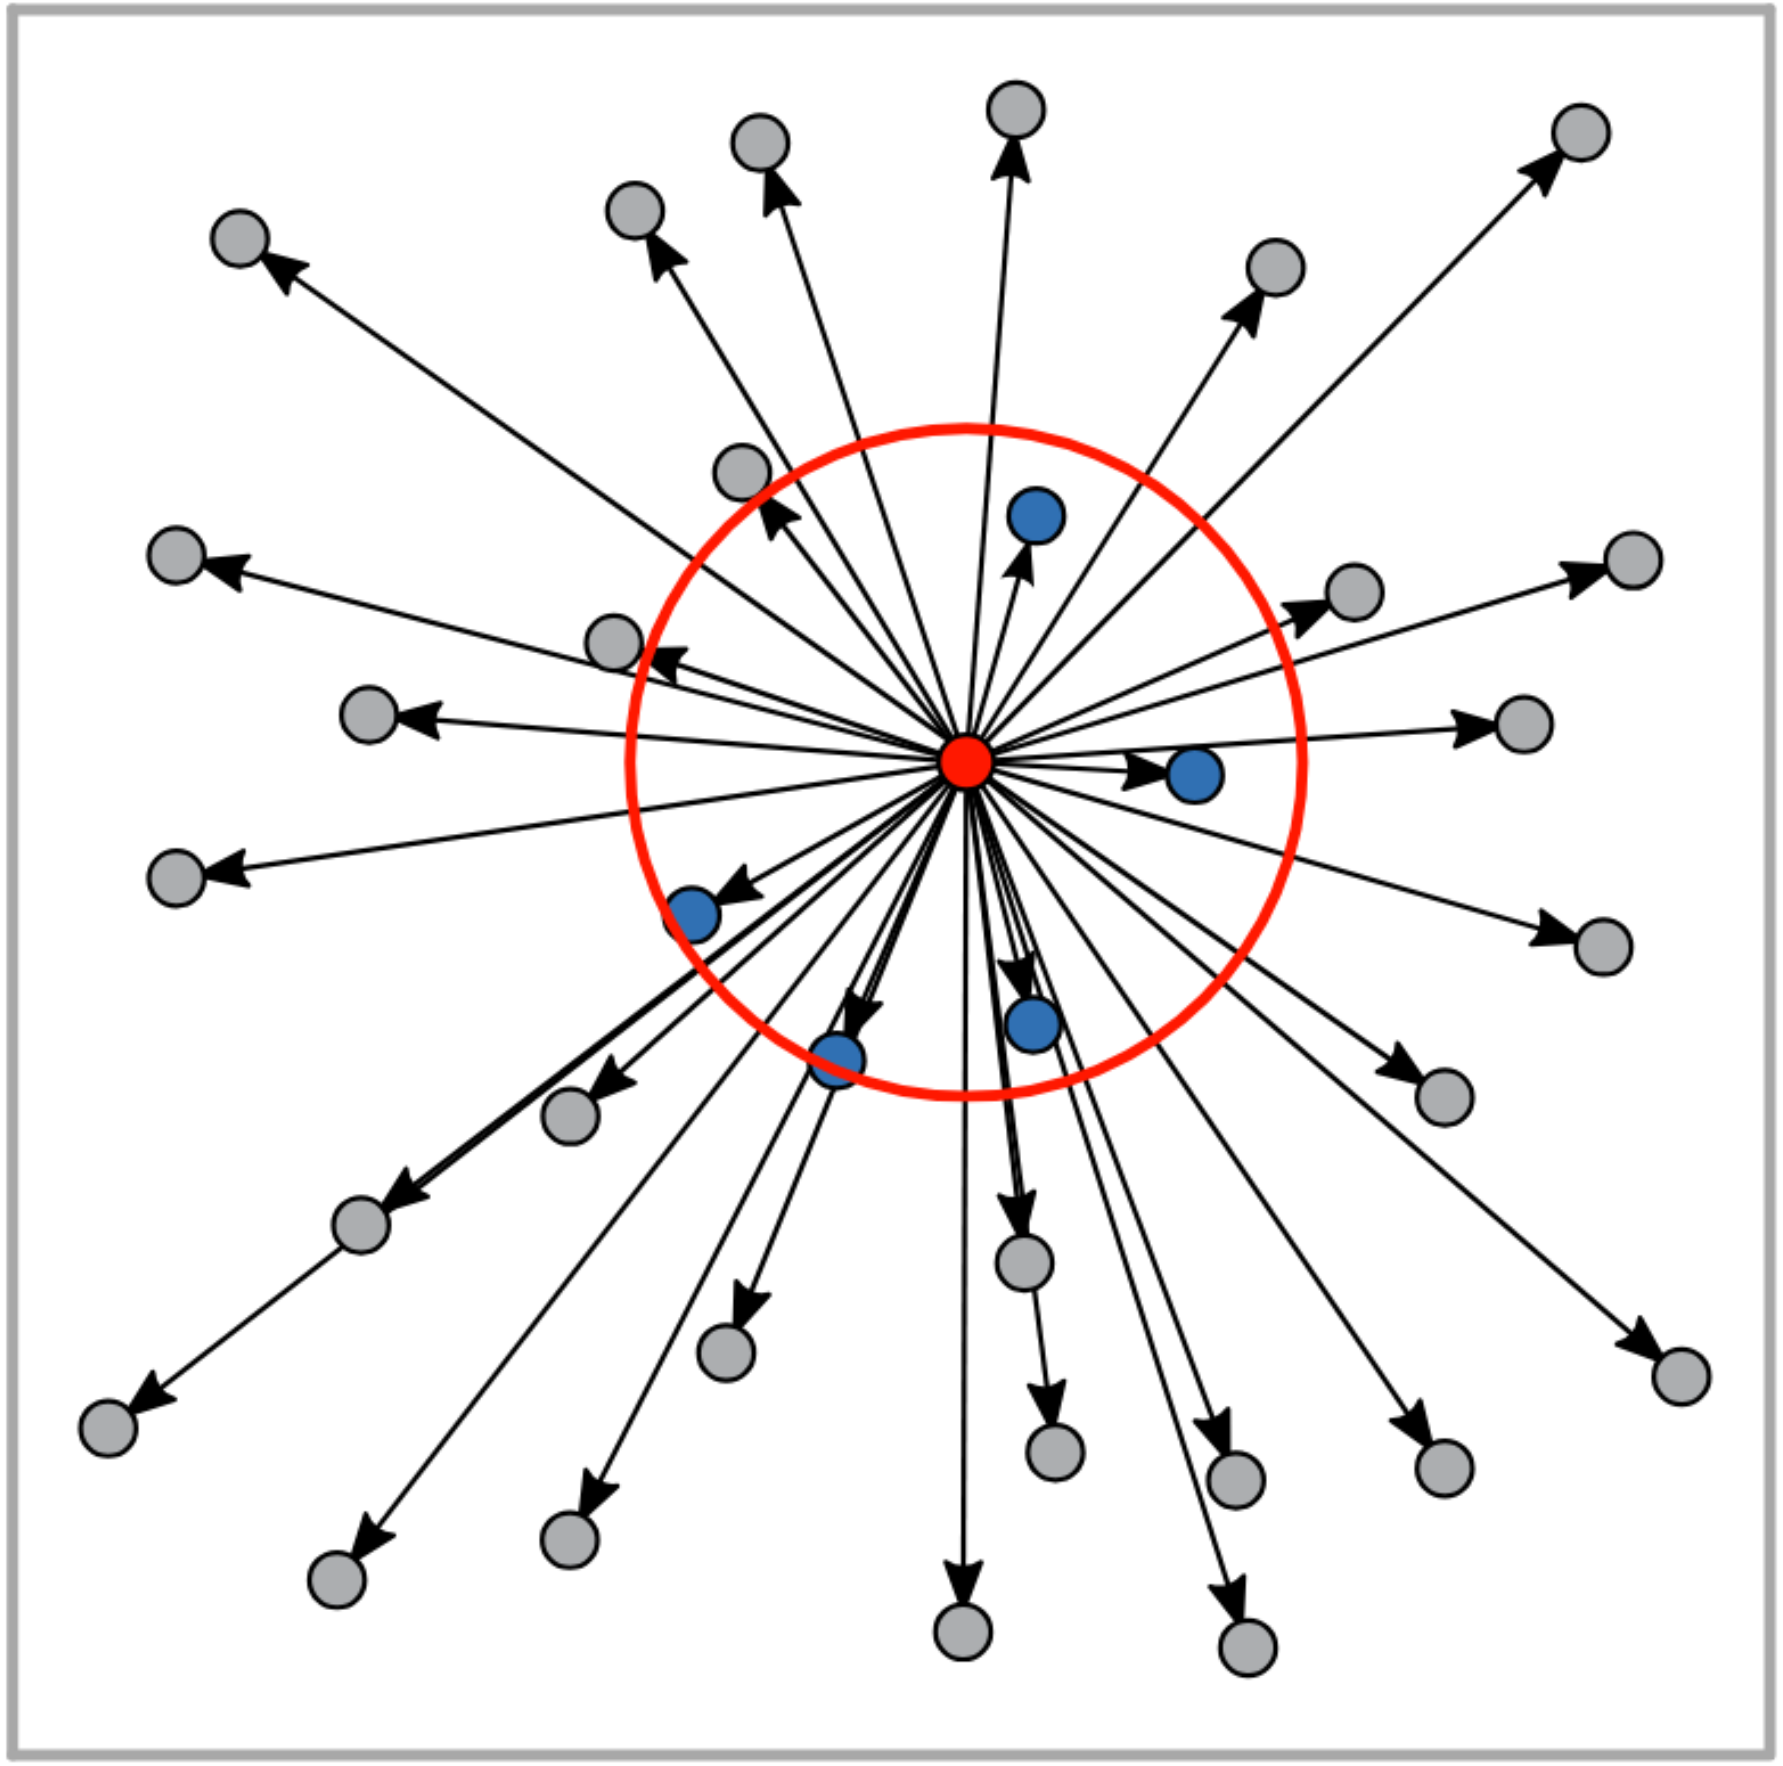
\includegraphics[width=\linewidth]{imgs/directsum.png}
        \caption{\scriptsize Direct Sum}
        \label{fig:directsum}
    \end{subfigure}
    \hfill
    % Second Figure
    \begin{subfigure}{0.22\textwidth}
        \centering
        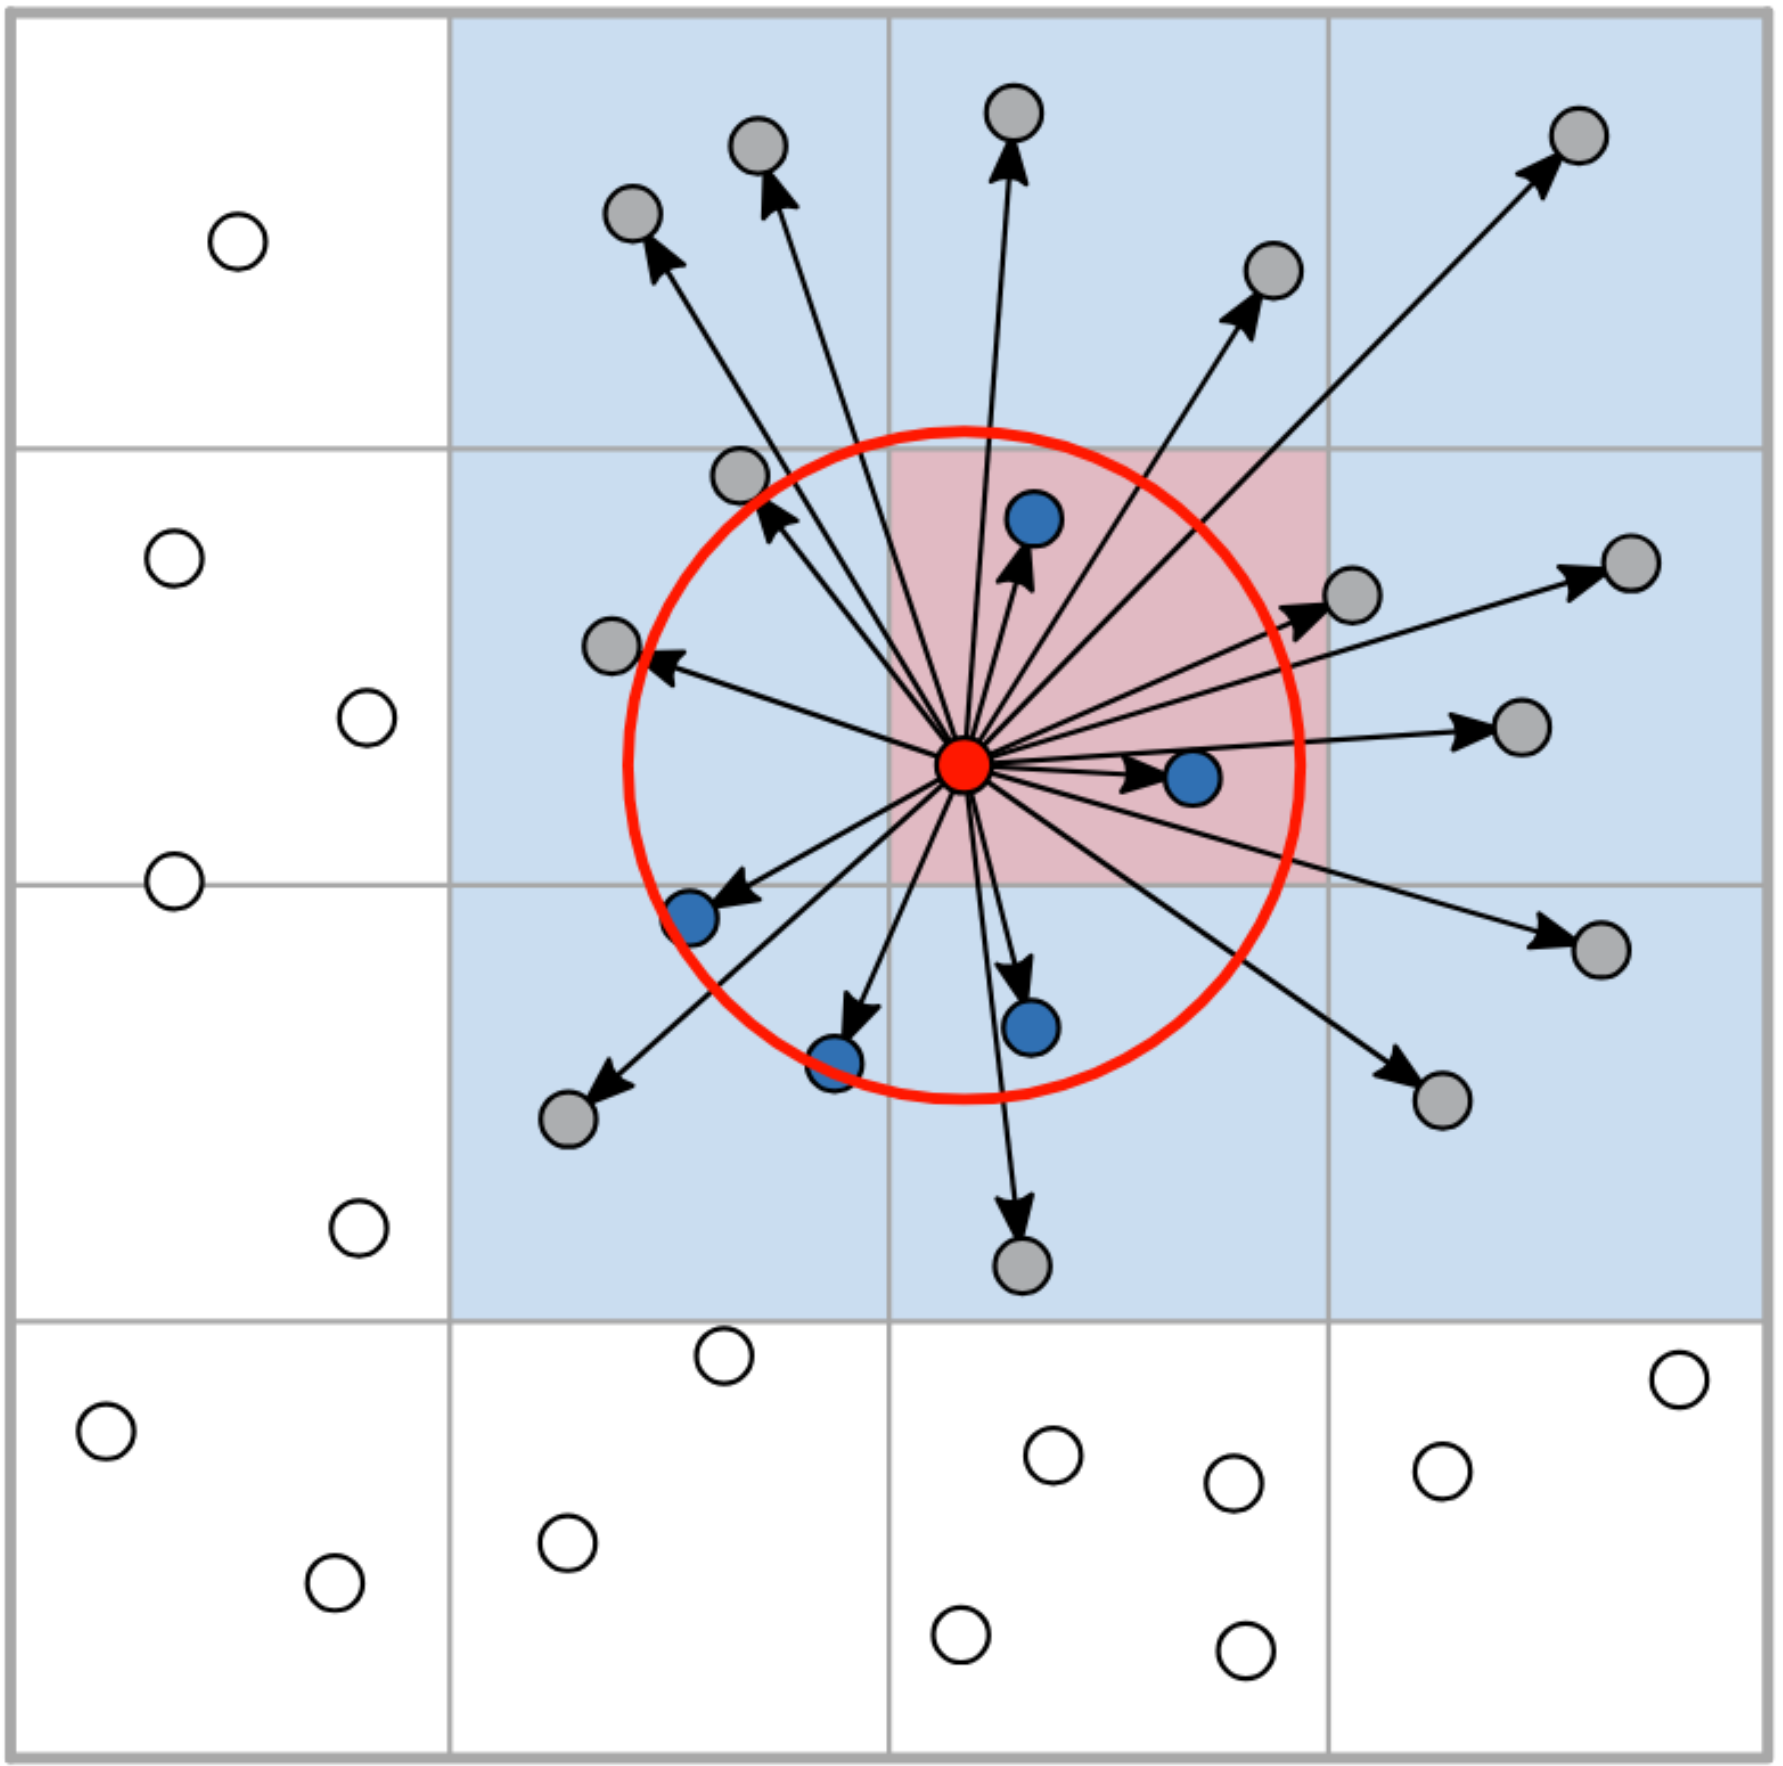
\includegraphics[width=\linewidth]{imgs/linkedcells.png}
        \caption{\scriptsize Linked Cells}
        \label{fig:linkedcells}
    \end{subfigure}
    \hfill
    % Third Figure
    \begin{subfigure}{0.22\textwidth}
        \centering
        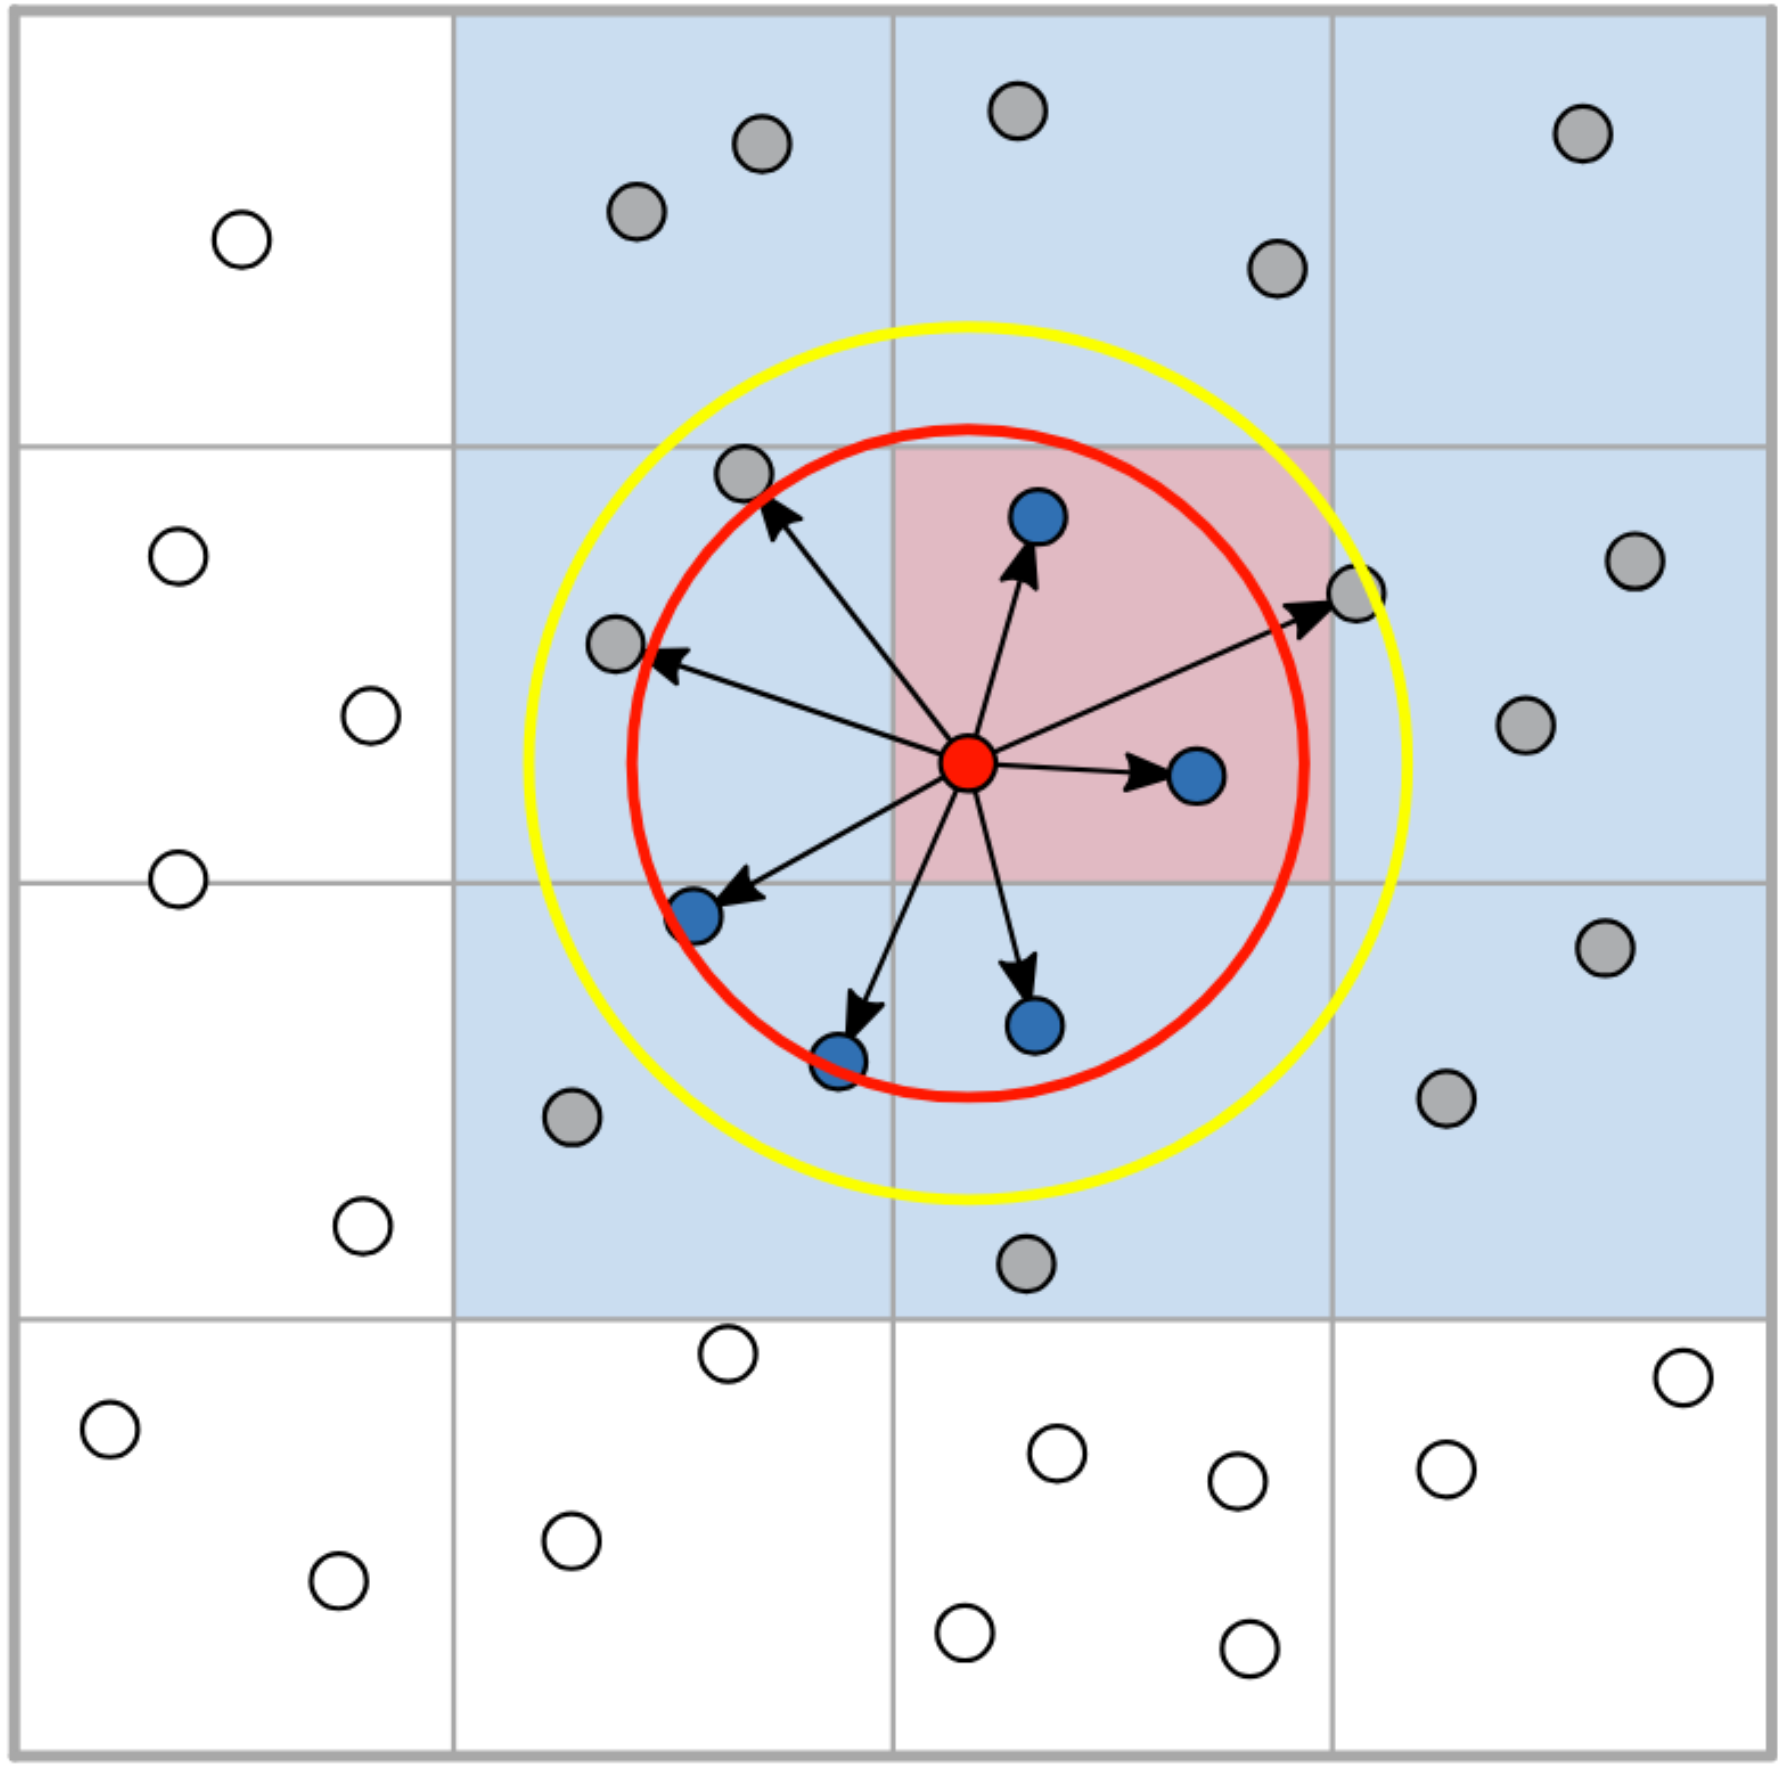
\includegraphics[width=\linewidth]{imgs/verletlists.png}
        \caption{\scriptsize Verlet Lists}
        \label{fig:verletlists}
    \end{subfigure}
    \hfill
    % Fourth Figure
    \begin{subfigure}{0.22\textwidth}
        \centering
        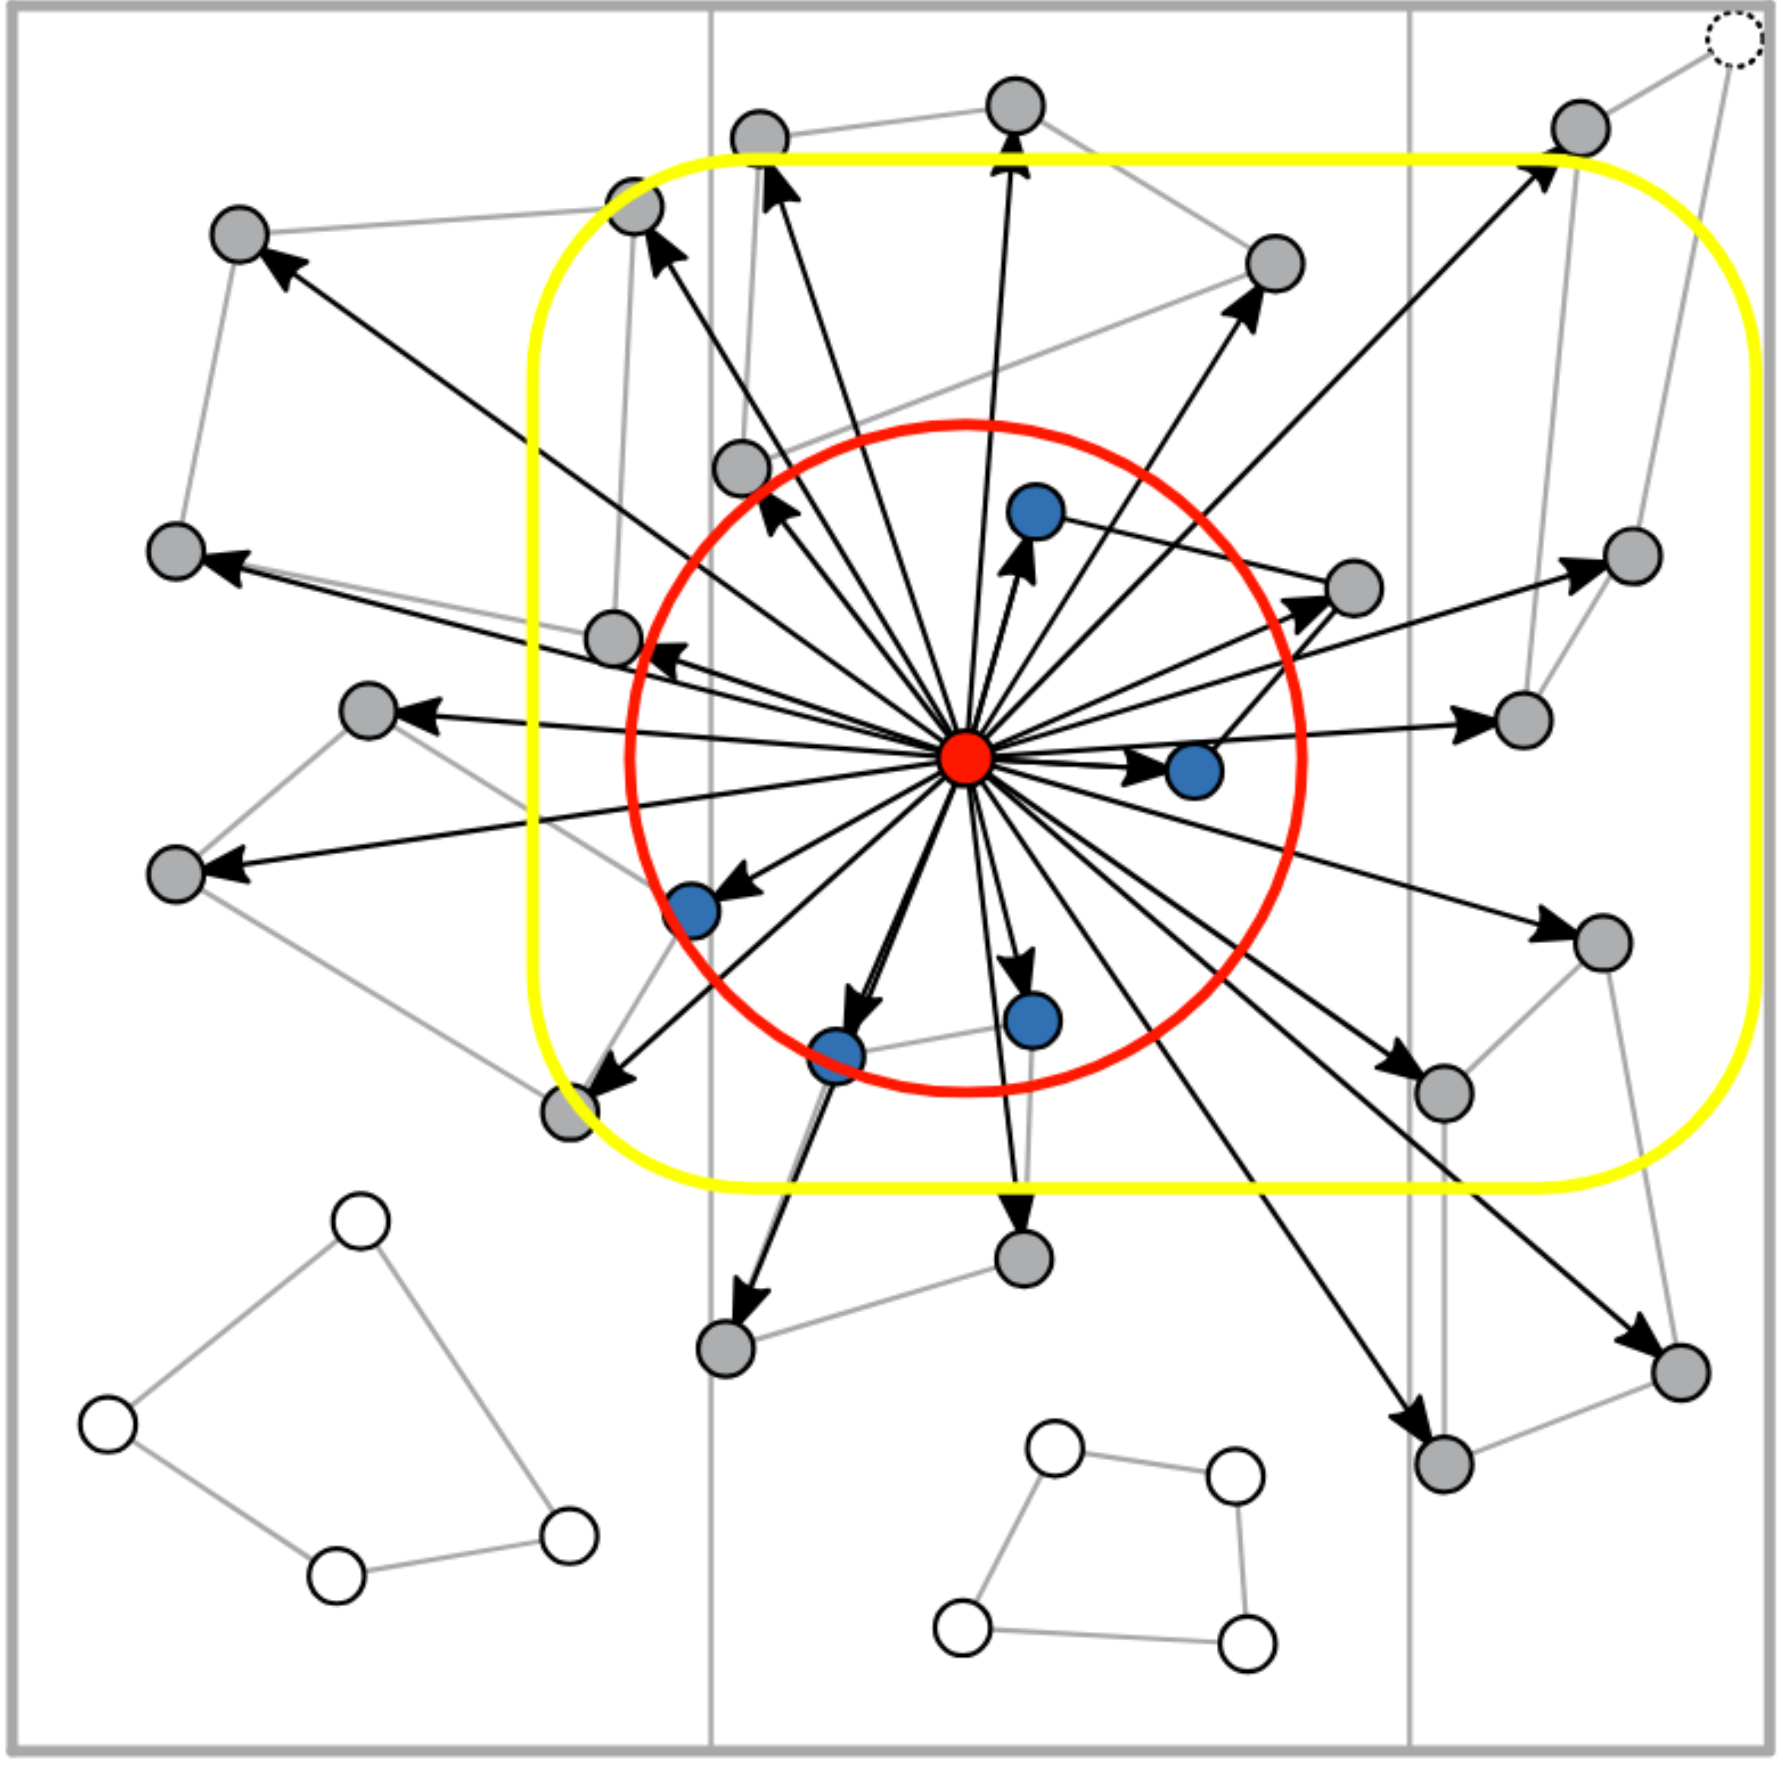
\includegraphics[width=\linewidth]{imgs/verletclusters.png}
        \caption{\scriptsize Verlet Cluster Lists}
        \label{fig:verletclusters}
    \end{subfigure}
    \caption{Neighbor identification algorithms \parencite{gratl2022n}}
\end{figure}



\subsection{Traversals}

Traversals play a crucial role in AutoPas, as they determine the order in which particle interactions are computed. AutoPas supports a variety of traversal strategies, each specific to the container being used. These strategies are designed to optimize performance by parallelizing the traversal process while avoiding race conditions and minimizing the need for schedulers or locking mechanisms \parencite{gratl2019autopas}.

Traversal strategies in AutoPas utilize different cell strategies as their base step. The goal of these base steps is to divide and color the cells of the domain, such that particles in cells of the same color can be processed independently by separate threads. Currently, AutoPas implements three types of base steps: c01, c18, and c08. 

\subsection{Base Steps in AutoPas}

\subsubsection{c01 Base Step} The c01 base step uses only a single color, as illustrated in Figure \ref{fig:c01}, and calculates interactions for all neighboring cells without utilizing the Newton3 optimization. In this approach, each cell is assigned to a thread, which calculates the interactions with particles in the neighboring cells. This strategy is highly parallelizable.

\subsubsection{c18 Base Step} The c18 base step assigns one of 18 colors to each cell, ensuring that no two neighboring cells share the same color. By utilizing the Newton3 optimization, the number of interactions to be calculated is reduced by half. Instead of processing all neighbors, it focuses only on neighbors with a higher index (see Figure~\ref{fig:c18}). This reduces the overall number of computations, however increases the area where race conditions need to be managed, limiting parallel execution.

\subsubsection{c08 Base Step} As the name suggests, the c08 base step uses 8 colors. It is similar to c18 but reduces the locked area further by limiting diagonal interactions and focusing on only four cells (see Figure~\ref{fig:c08}). This adjustment allows for better parallel processing and improved cache utilization.


\subsection{Traversal Strategies}
This thesis focuses on the traversals \texttt{lc\_c08}, \texttt{vlc\_c08}, and \texttt{vcl\_c06}, as they were extensively used in the experiments conducted. A detailed explanation of these strategies is provided below. For information on all traversal strategies, refer to \parencite{gratl2022n}.

\subsubsection{\texttt{lc\_c08}}
This traversal utilizes \texttt{c08} as its base step, and it is designed for the Linked Cells container. It divides a 2D domain into four colors and a 3D domain into eight colors. The dependency of the number of colors \(C\) on the number of dimensions \(D\) follows \(C = 2^D\) \parencite{gratl2022n}.

\subsubsection{\texttt{vlc\_c08}}
This traversal applies the \texttt{c08} base step to each individual cell. To ensure thread safety, a domain coloring consisting of eight colors is used. For each cell, all neighbor lists are processed. Depending on whether the lists were built with Newton3, the base step used is either c01 or c08. \parencite{AutoPasDocs}

\subsubsection{\texttt{vcl\_c06}}
This traversal is used for VerletClusterLists and it employs a 2D coloring scheme with a stride of \(x = 3\) and \(y = 2\), resulting in six colors (\(3 \times 2 = 6\)). Interactions within clusters are always computed using Newton3, regardless of whether Newton3 is enabled or disabled for the overall traversal. \parencite{AutoPasDocs}

\begin{figure}[htbp]
    \centering
    \begin{subfigure}[b]{0.3\textwidth}
        \centering
        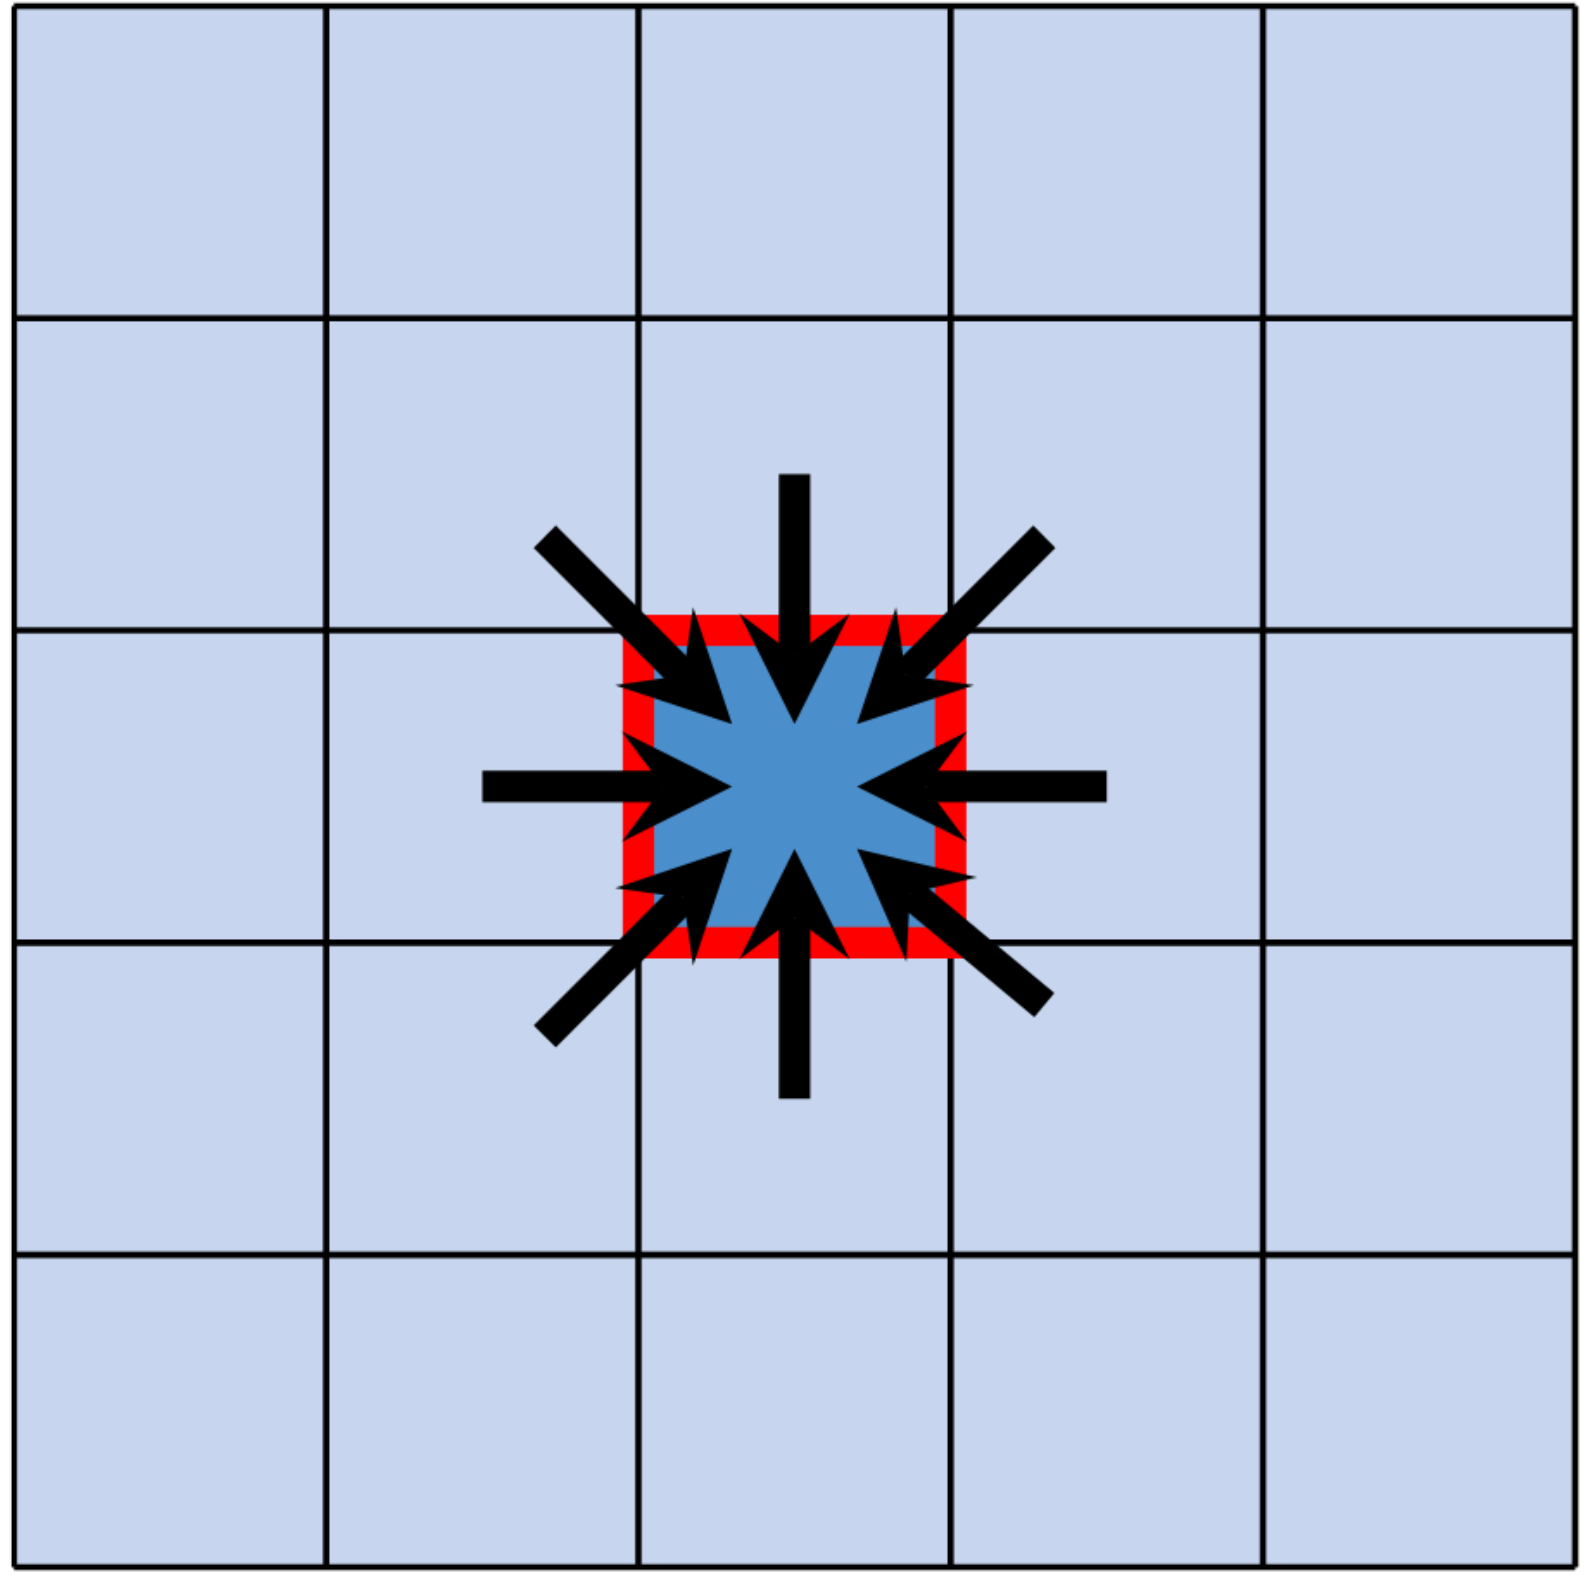
\includegraphics[width=\linewidth]{imgs/c01.png}
        \caption{\scriptsize c01 base step}
        \label{fig:c01}
    \end{subfigure}
    \begin{subfigure}[b]{0.3\textwidth}
        \centering
        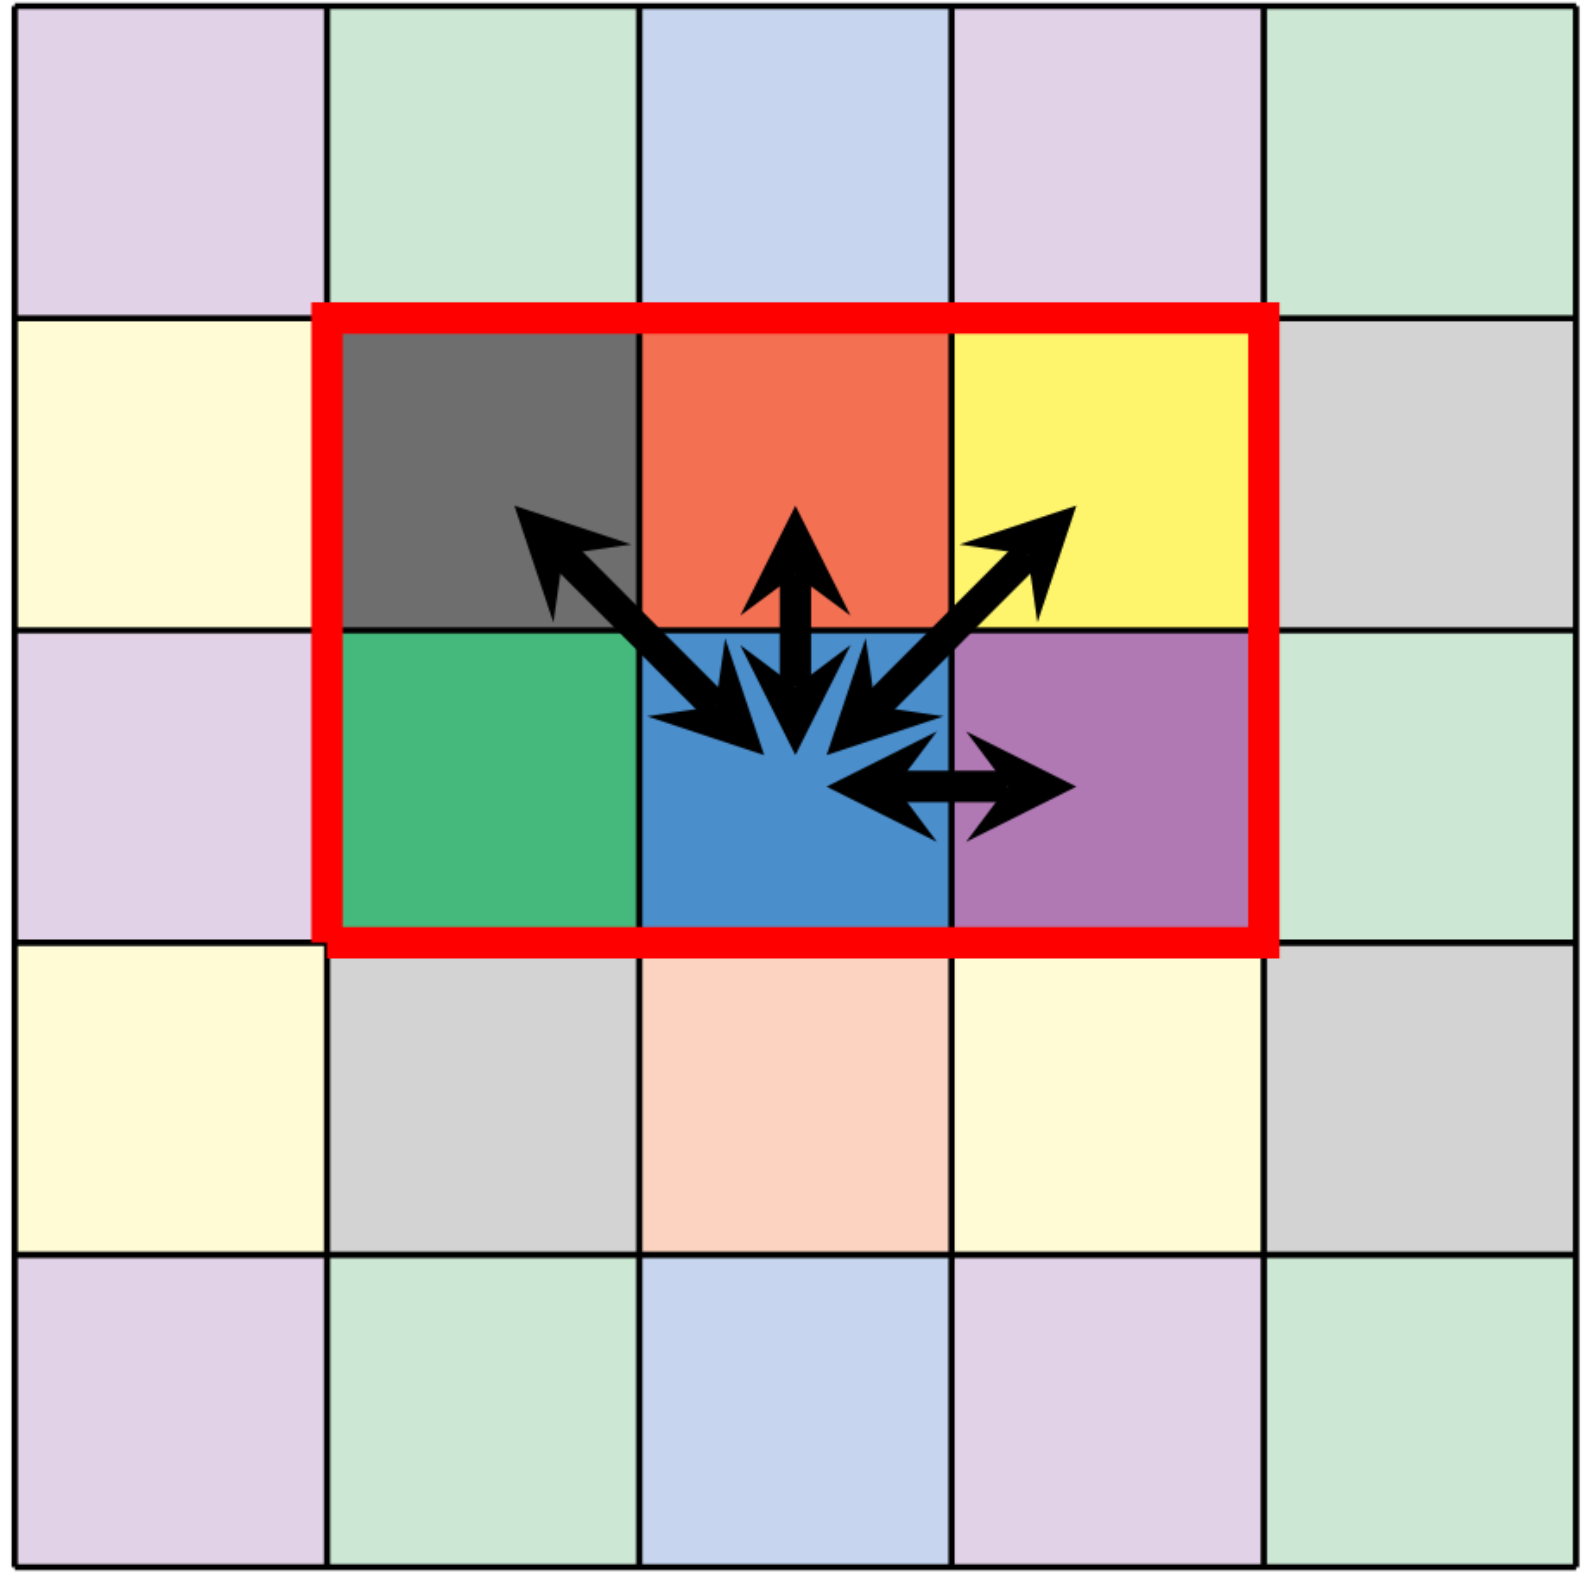
\includegraphics[width=\linewidth]{imgs/c18.png}
        \caption{\scriptsize c18 base step}
        \label{fig:c18}
    \end{subfigure}
    \begin{subfigure}[b]{0.3\textwidth}
        \centering
        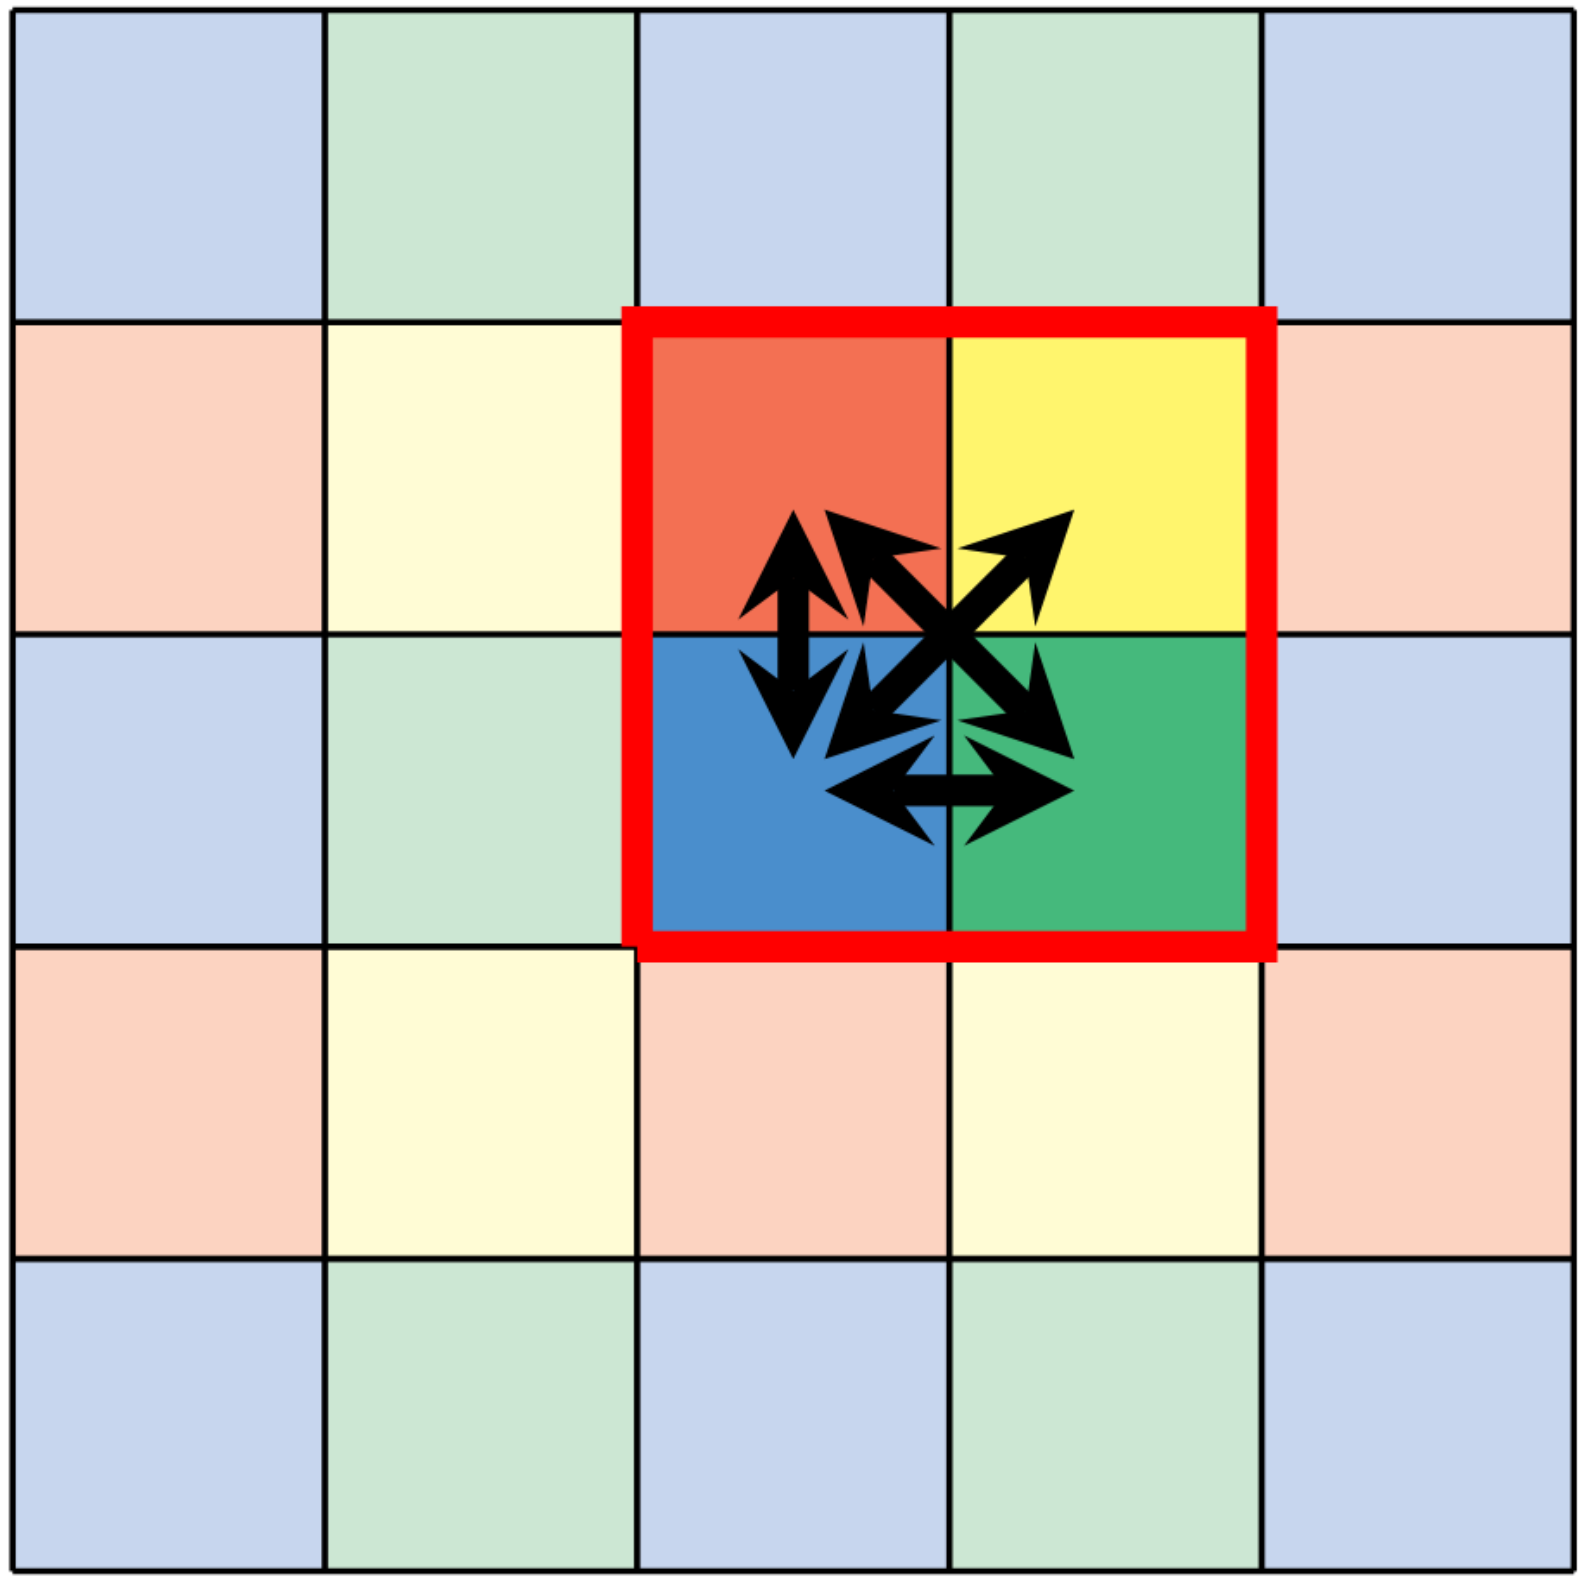
\includegraphics[width=\linewidth]{imgs/c08.png}
        \caption{\scriptsize c08 base step}
        \label{fig:c08}
    \end{subfigure}
    \caption{Base Steps Approaches \parencite{newcome2023towards}}
\end{figure}



\subsection{Auto-Tuning}

One of the key features of AutoPas is its auto-tuning capability. Choosing the optimal combination of container and traversal for a simulation can be challenging, especially since different parts of the simulation may benefit from different configurations. AutoPas automates this process, relieving the user of the need to determine the best setup manually.

At the beginning of a simulation, AutoPas tests various configurations over a few iterations, measuring their performance. To reduce overhead, configurations using the same container are tested consecutively. This approach assumes that the state of the simulation remains relatively stable over consecutive time steps, making the performance results comparable. Importantly, the results of these initial tests are not discarded but are used to guide the following iterations \parencite{gratl2019autopas}.

After evaluating multiple configurations, AutoPas selects the best-performing setup and uses it for a user-defined number of iterations. Following this period, the system enters a re-tuning phase, where new configurations may be selected based on how the simulation has evolved.

